%! TEX root = ../main.texslm
\documentclass[../main.tex]{subfiles}
\begin{document}
\section{Verfahren}
\subsection{Selective Laser Melting}
\acrfull{slm} verwendet weiterhin Grundelemente des SLA, namentlich den Laser und ein Substrat, welches durch den Laser zusammengefügt wird zu einem fertigen Bauteil. 
Jedoch wird die Wellenlänge des Lasers vom UV-Bereich (\qty{0.01}{\micro\meter} bis \qty{0.38}{\micro\meter}) in den Infrarot-Bereich bei in etwa \qty{1.06}{\micro\meter}-\qty{1.08}{\micro\meter} verschoben, was auf die höhere Energie-Adsorption von Stählen im IR-Bereich zurückzuführen ist.\parencite{3FAKTUR_1}
\begin{figure}[h]
\begin{center}
	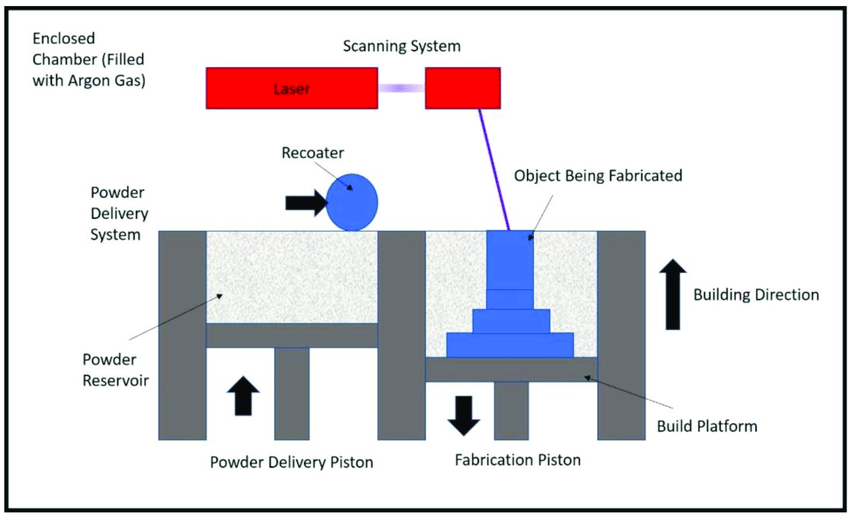
\includegraphics[width=.5\textwidth]{slm_diagram}
	\label{img:slm_diagram}
	\ccaption{Schematischer Aufbau einer SLM-Maschine}{\url{https://www.researchgate.net/publication/326891428/figure/fig1/AS:659597278855194@1534271654724/Schematic-diagram-of-the-selective-laser-melting-SLM-process.png}}
\end{center}
\end{figure}	
SLM ist ein Schichtverfahren, was daran erkennbar ist, dass es Schicht für Schicht ein Bauteil aufbaut wie ein konventioneller Kunststoff-Drucker. Dies passiert auf einer Bauplattform, welche nach jeder Schicht sich um die eingestellte Schichtdicke nach unten bewegt, um das Auftragen einer neuen Schicht zu ermöglichen. 
Hinzu kommt, dass SLM ein Pulverbett-Verfahren ist, was wiederum bedeutet, dass eine neue perfekt ebene Schicht auf dem Baustück aufgetragen werden muss nach jedem Absenken der Plattform mithilfe eines Wiederbeschichtungswerkzeugs.
Dieser ist meist ein Roller oder ein Kunststoff-Schieber. Nach jeder Absenkung des Druckbettes wird über die Pulverlieferungsplatte Baumaterial nachgeliefert, welche dann vom Wiederbeschichtungswerkzeug eben verteilt wird am Druckbett. Der Exzess wird aufgefangen und gesiebt, um die Verschwendungsrate gering zu halten.  
Die Distanz des Wiederbeschichtungswerkzeugs zum Druckbett bestimmt die Schichtdicke, welche große Auswirkungen auf den Teil hat. Eine höhere Schichtdicke (über \qty{50}{\micro\meter}) führt zu schnellerer Produktionszeit, aber das produzierte Teil benötigt daraufhin mehr Nachbearbeitung durch verschiedene Verfahren wie Drehen, Polieren und Schleifen, um die korrekten Dimensionen zu garantieren. Allgemein wird dieser Geschwindigkeits-Vorteil gerne ignoriert, um die Nachbearbeitung zu ersparen, da bei dieser immer Fehler passieren können, welche das Bauteil unbrauchbar machen können.

\end{document}
